\chapter{Methodologies}
\graphicspath{{Chapter3/Figs/}{Chapter3/Figs/}}

This chapter describes the project-related academic methodologies in the author's given context and the planned approach to achieve the thesis's goals and objectives. The reader is introduced to the rationale for the intended workflows, hardware, and software tools.

\section{Derivation of the case study}
\label{chapter3-derivation-of-the-case-study}

In October 2021, the author began working as a cloud software engineer at IDUN Technologies with the intention of further developing the existing software products. IDUN Technologies had already created a PoC software system that included a web-based single-page application (SPA) hosted on AWS Amplify, an backend-as-a-service that aims at simplifying the deployment of backends for mobile or web apps. IDUN's in-ear headphone sensor sent EEG data to a network bridge via Bluetooth and then to the cloud via the internet. The raw EEG data was saved and made available for download in a variety of file formats.

\begin{figure}[!ht]
  \centering
  
\includegraphics[width=\linewidth]{raw-filtered-data.png}
  \caption{Difference between raw and filtered EEG data from IDUN's in-ear device.}
  \label{fig:raw-filtered-eeg}
\end{figure}

In addition to raw data, the IDUN app provided transformed data, such as e.g. filtered data, which included low-pass and high-pass filtering of EEG data as shown on \autoref{fig:raw-filtered-eeg}. This transformed EEG data was then saved alongside the raw version on the cloud. The EEG data could also be visualised in near-real time on the web app as a time-series x- and y-axis plot. Additionally, users could control the device by sending start and stop commands to the hardware components. The overview of the architecture is displayed on \autoref{fig:idun-amplify}.

\begin{figure}[!ht]
  \centering
  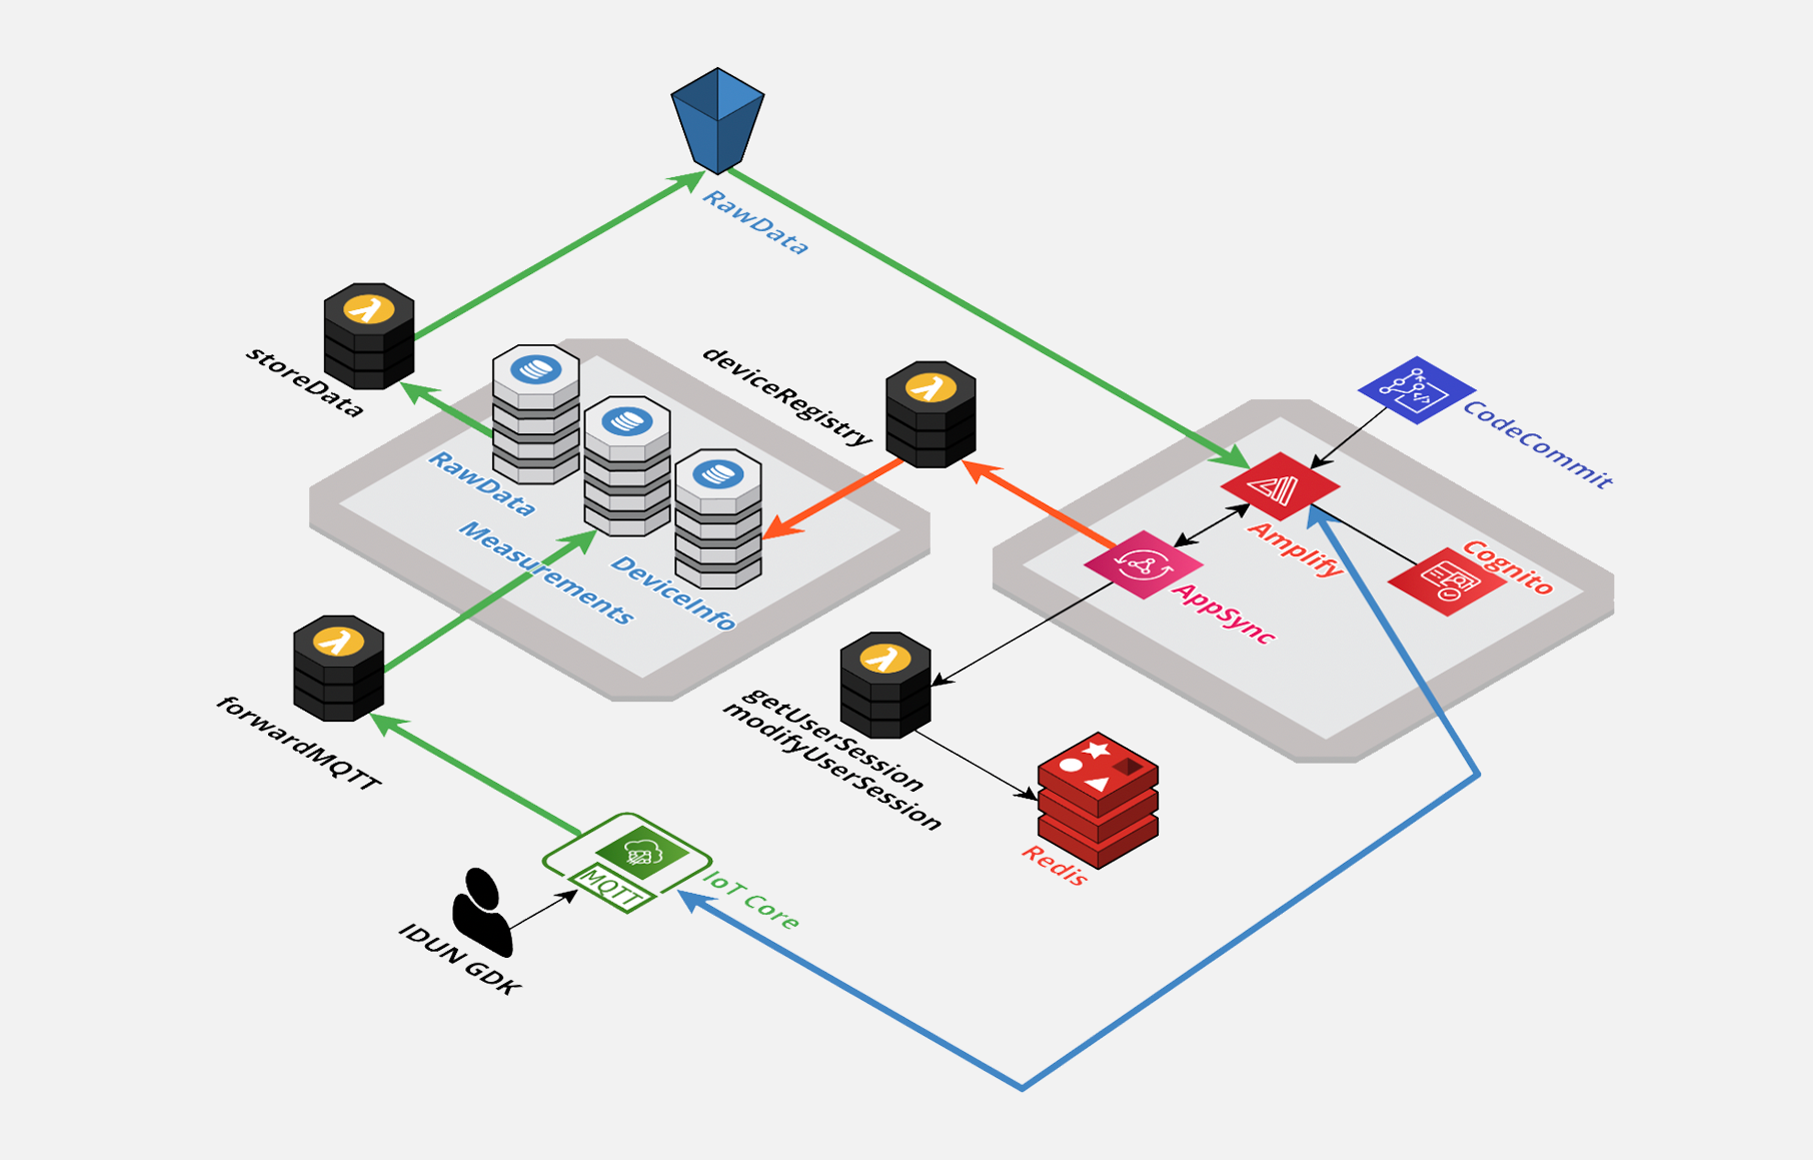
\includegraphics[width=\linewidth]{idun-amplify.png}
  \caption{IDUN's software architecture at the end of 2021.}
  \label{fig:idun-amplify}
\end{figure}

The system itself was in a rather unstable state and had strange error sources that made it impossible to reliably record EEG data for more than a few minutes, making the product unusable for a current customers or in general for a mass-market launch. While working on the system, the author encountered a various amount of technological flaws as listed in the following list:

\begin{enumerate}
  \item AWS Amplify is great for simple backends with CRUD\footnote{CRUD is an acronym describing general operations of a backend system: Create, Read, Update and Delete.} but not so great for everything custom-made such as the streaming-focused aspect of EEG. Therefore, the need to break out of the AWS Amplify system would either way need to happen anytime soon since it would otherwise be building a project with the wrong tools and foundations.
  \item The network bridge was a Raspberry Pi running Python code which, after some analysis turned out to be the main source of most bugs. The question was raised if the network bridge was even needed, as IDUN either way would go into being a fully-mobile system rather than network bound and therefore aiming at being connected directly to a mobile phone or computer.
  \item The heartbeat functionality of the cloud was missing, which basically meant that the cloud did not know anything about the hardware devices, it just assumed that data would flow in as soon as the start command was sent to the device, therefore having a happy-path-only scenario. There were many happy path scenarios present.
   \item The infrastructure of the application was automatically provided by AWS Amplify and used AWS CloudFormation under the hood inside AWS CodePipeline which is AWS's own continuous integration service. The entirety of the software on the cloud was built via the AWS Console (the GUI of AWS) and therefore there was no current state in form of code to reflect the current infrastructure, ergo making reproducibility of the cloud impossible.
   \item The streaming of the data happened through MQTT, a publish and subscribe-based protocol usually used for Internet of Things (IoT) devices such as sending periodically health checks. The intent of MQTT was not the real-time sending of EEG data, therefore the need was also there to reconsider this technological decision which was deeply rooted into another AWS service called IoT Core.
   \item The end-user of the software product was also still uncertain, therefore making it even harder to define what the system should actually be able to achieve. IDUN needed to figure out if the software system is rather aimed at researchers, developers, end-users etc. The priorisation of the engineering roadmap was therefore uncertain.
   \item The web app was a thick client and did not consume one single API endpoint from the AWS backend. Thick client means that the web app did quite a lot of business logic, such as the filtering of the raw data for the near-realime visualisation which was another technological misdecision since the client-side JavaScript ecosystem is way far inferior compared to e.g. the Python ecosystem which could run on the backend.
   \item The web app was not connected to a single endpoint on the backend and consumed the MQTT stream and non-real-time aspects of the app (login, list recorded EEG data and so on) via different sources. E.g. the MQTT stream was directly subscribed from the device itself via AWS IoT Core and did not go through the GraphQL API from AWS Amplify, which made coupling the systems to a cohesive and robust API tedious.
\end{enumerate}

Due to growing problems with the existing software system and an ever-increasing technical debt as a result of the software not being test-driven or developed without code quality standards, resulting in bugs and quirks that are difficult to track down, the author proposed to halt the implementation of new functions and restructure the system from the ground up using a more software engineering oriented approach. The company's management approved the request in for such a redevelopment.

The author was already working on his original Bachelor project, which focused on a mind-controlled multiplayer game, assuming that IDUN's software system would be stable by the time the Bachelor project began. The original bachelor project's focus was officially changed at the end of 2021 to creating this refactored software system.

\section{Case study}
\label{chapter3-case-study}

A possibility to conduct research in order to build a N/CI with the assumed requirements as defined with the three-dimensionality was to do a case study at the research and development (R\&D) team at IDUN Technologies.

% Forty-three patients of the psychiatric clinic with diagnosed major depression (12 male, Mage = 36.35, SDage = 7.92) participated in this study for monetary compensation (10 USD).

\section{Procedure}
\label{chapter3-procedure}

\subsection{Project stages}
\label{chapter3-project-stages}

% - The study used a between-subject design (treatment group, control group) with the
% depression score on the XXX depression scale as dependent variable.
% - The study used a within-subject design (pre-treatment measurement, post-treatment
% measurement) with the depression score on the XXX depression scale as dependent variable.
% - The study used a mixed design with the between-subject factor group (treatment, control) and the within-subject factor time (pre-treatment, post-treatment). The depression score on the XXX depression scale served as the dependent variable.

% - Three types of materials were used. First,… Second,… Third,…

% - Before the experiment started, participants were randomly assigned to two groups: the X group and the Y group.
% - The experiment consistent of two phases. In the first phase,….. . In the second phase,…. .
% - The order of these two phases was counterbalanced
% - First, participants had to… next… subsequently… finally…
% - Simultaneously,…
% - After participants finished X, they… % Example citation

\subsection{Group discussions}
\label{chapter3-group-discussions}

\subsection{Expert interviews}
\label{chapter3-expert-interviews}

\section{Outcomes}
\label{chapter3-outcomes}

\section{Reflection}
\label{chapter3-reflection}

\section{Further development}
\label{chapter3-further-development}

% - First, they were randomly assigned to treatment and placebo group
% - Both groups: 60 minutes intervention
% - Treatment group: first,… next,…
% - Placebo group: first, …next,…
% - Finally, they filled out the depression questionnaire
% o Did you describe everything that is needed to replicate your research?
% o Did you cite the sources of your methods or paradigms?

\nomenclature[rd]{R\&D}{Research and development}
\nomenclature[nip]{NIP}{Neuro-Intelligence Platform}
\nomenclature[spa]{SPA}{Single-page application}
